%====================================================================================================
% FaultRecovery: A ampliação da biblioteca de tolerância a falhas
%====================================================================================================
% TCC
%----------------------------------------------------------------------------------------------------
% Autor				: Cleiton Gonçalves de Almeida
% Orientador		: Kleber Kruger
% Instituição 		: UFMS - Universidade Federal do Mato Grosso do Sul
% Departamento		: CPCX - Sistema de Informação
%----------------------------------------------------------------------------------------------------
% Data de criação	: 10 de Maio de 2016
%====================================================================================================

\chapter{Resultados} \label{cap:Resultados}

Neste capítulo são apresentados os resultados dos testes realizados. 

\section{Desempenho da Biblioteca \textit{FaultRecovery}} \label{Sec:tempoRecovery}

Esta seção tem como objetivo demonstrar o desempenho da biblioteca \textit{FaultRecovery} em termos de tempo de execução. Para realizar os testes, utilizou-se cinco algoritmos de ordenação \textit{bubble sort, insertion sort, merge sort} e \textit{comb sort} \cite{orderUnicamp, vivaLinux}, a execução dos cinco algoritmos forma um ciclo de teste. Ao todo cada ciclo foi executado cem vezes. Os algoritmos foram implementados para ordenar os elementos em forma crescente em um microcontrolador \textit{mbed} LPC1768. Para cada ciclo de teste, utilizou-se um vetor do tipo \textit{unsigned short} contendo 4096 elementos enumerados em ordem decrescente de $n$ (4096) até 1, ou seja, o elemento da primeira posição recebeu o valor $n$, da segunda $n-1$, e assim sucessivamente até o elemento da última posição receber o valor 1. Essa estratégia foi utilizada para que o tempo de execução dos algoritmos fosse similar, pois se o vetor estivesse com números aleatórios ao invés de decrescente, isso poderia afetar o comportamento dos algoritmos. Por isso tentou-se manter um padrão para que fosse possível medir o tempo da biblioteca. O tamanho total do vetor totalizou 8kB de memória (2 bytes * 4096). Tentou-se aumentar a quantidade de elementos do vetor, entretanto quando se tentou alocar um espaço de memória maior que 8kB, o \textit{firmware} teve sua execução interrompida no primeiro ciclo de teste, em outros no segundo.

O primeiro teste teve como objetivo medir o tempo de execução dos algoritmos de ordenação, simulando um \textit{firmware} implementado por um usuário que não utilizou a biblioteca \textit{FaultRecovery}. Todos os algoritmos compartilharam do mesmo vetor, por isso, antes de cada ordenação foi necessário desordenar o vetor para cronometrar o tempo real de ordenação. O tempo de cada algoritmo foi cronometrado, desde o início de sua execução até seu fim, sendo desprezado o tempo de desordenação do vetor.

O segundo teste teve como objetivo medir o tempo de execução dos mesmos algoritmos de ordenação, fazendo uso da biblioteca \textit{FaultRecovery}. O tempo de execução no segundo teste foi medido a partir do início da execução de um estado da máquina de estados até o fim dele. Tanto para o primeiro quanto para o segundo teste foi utilizada a mesma quantidade de elementos do vetor (4096), a mesma sequência de execução (\textit{bubble, insertion, selection, merge} \textit{e comb}) e o tempo de desordenação do vetor também foi desprezado. Ao final das cem execuções do primeiro e do segundo teste, as médias de tempo de execução para cada algoritmo e para cada ciclo de teste foram calculadas. O tempo de execução da biblioteca \textit{FaultRecovery} também foi calculado, obtendo-se o resultado mostrado na Figura \ref{Img:tempoRecovery}.

\begin{figure}[h]
	\centering
	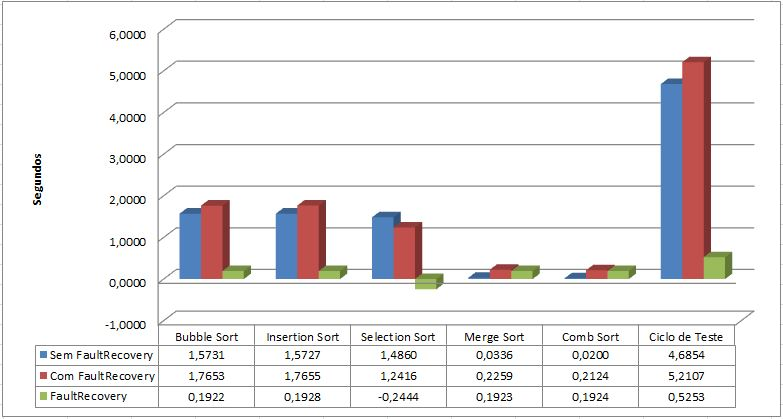
\includegraphics[width=0.9\textwidth]{figuras/tempoRecovery.jpg}
	\caption[Tempo de execução da biblioteca \textit{FaultRecovery}]{Nesta figura são mostrados os resultado dos testes de medição do tempo de execução dos algoritmos de ordenação, sem a biblioteca e com a biblioteca. Percebe-se que com a utilização da biblioteca o tempo de execução dos algoritmos aumentou em média 0,5253 segundos ou 525,3 milisegundos.}
	\label{Img:tempoRecovery}	
	%width=0.5\textwidth (Tamanho da Imagem)
\end{figure}	
\newpage
Dentre os tempos de execução mostrados na Figura \ref{Img:tempoRecovery}, obteve-se um resultado inesperado: o tempo de execução do algoritmo \textit{insertion sort} foi menor com a biblioteca \textit{FaultRecovery}, mesmo ela gerando maior de execução (devido à gerência da estrutura de sua máquina de estados). Diante disso, verificou-se a implementação dos dois testes, e não foi constatada nenhuma diferença entre os códigos que pudessem causar este resultado. Então, um terceiro teste foi executado outras cem vezes, utilizando-se um vetor de 6KB (menor que o utilizado nos testes anteriores) para verificar se comportamento anômalo persistiria em ocorrer. O resultado foi similar, ou seja, o comportamento persistiu, mas como não havia tempo hábil para uma análise aprofundada, presumiu-se que esses casos são factíveis de ocorrer, provavelmente devido as otimizações de código feitas pelo compilador, já que o microcontrolador utilizado nos testes não possui sistema operacional e nenhuma outra aplicação rodando simultaneamente. Portanto verificou-se que quanto maior o volume de dados do vetor, o tempo de execução da \textit{FaultRecovery} torna-se menos expressivo. Os resultados do terceiro teste são mostrados na Figura \ref{Img:tempoRecovery2}.

\begin{figure}[h]
	\centering
	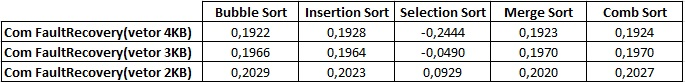
\includegraphics[width=0.9\textwidth]{figuras/tempoRecovery2.jpg}
	\caption[Tempo de execução da biblioteca \textit{FaultRecovery} com três tamanhos de vetores diferentes.]{Nesta figura é mostrado o tempo de execução da biblioteca \textit{FaultRecovery} com três vetores de tamanhos diferentes. Percebe-se que o tempo de execução da biblioteca no algoritmo \textit{insertion sort} é negativo no primeiro e no segundo teste, contudo no teste com o vetor de tamanho 4KB obteu-se um tempo de execução positivo. Portanto verificou-se que quanto maior o volume de dados do vetor, o tempo de execução da \textit{FaultRecovery} torna-se menos expressivo.}
	\label{Img:tempoRecovery2}	
	%width=0.5\textwidth (Tamanho da Imagem)
\end{figure}
\newpage
\section{Desempenho e Eficiência da Classe TData} \label{Sec:tempoTData}

Para testar a eficácia e o desempenho da classe \textit{TData} foram realizados dois tipos de testes. O primeiro não utilizou a classe \textit{TData} e o segundo a utilizou. Em ambos o vetor foi preenchido de forma decrescente e foram realizados cem ciclos de execução, conforme descrito no primeiro parágrafo da Seção \ref{Sec:tempoRecovery}. No entanto houve a necessidade de reduzir o tamanho do vetor de 4096 para 1024 elementos, devido à redundância de dados da classe \textit{TData}, pois ela copia um valor para três endereços de memória diferentes. Se fossem utilizados os 4096 elementos, a quantidade de memória alocada seria de aproximadamente 32kB, pois cada elemento que antes ocupava 2 bytes, passaria  utilizar 8 bytes. Isso impossibilitaria a realização dos testes. 


O primeiro teste, que não utilizou a classe \textit{TData}, teve como objetivo medir o tempo de execução de cada algoritmo de ordenação. Nele, a biblioteca \textit{FaultRecovery} não foi utilizada, foi levado em conta apenas o tempo de execução de cada algoritmo. O resultado do primeiro teste foi comparado ao do segundo, obtendo-se o tempo de execução conforme mostrado na Figura \ref{Img:tempoTData}. Para iniciar o segundo teste, foi necessário apenas substituir a declaração do vetor de \textit{unsigned short vetor[n]} para \textit{TData$<$unsigned short$>$ vetor[$n$]}, isso mostra que a \textit{TData} aplica redundância de dados de forma simples, reduzindo a reescrita de várias linhas de código.

Conforme exibido na Figura \ref{Img:falhaTData}, o teste sem a \textit{TData} para a quantidade de falhas acima de 10\% foi de 20\% para cada ciclo de testes. Com a \textit{TData} esse número caiu para zero. Em contrapartida, notou-se uma diferença média de 0,2658 segundos a mais no tempo do ciclo com redundância de dados. 

Foram determinados três parâmetros de teste para deliberar se um ciclo de teste falhou ou não. Como o vetor possuía 1024 elementos ordenados em ordem decrescente de $n$ até 1, o resultado de uma ordenação crescente é conhecido. Após a injeção de falhas no microcontrolador \textit{mbed}, alterando um endereço de memória aleatório, estabeleceu-se que para um ciclo de teste falhar ele deveria ter entre 10\%, 25\% ou 50\% dos 1024 elementos diferentes do resultado conhecido. Essa estratégia foi utilizada para se ter uma medida reduzida (10\%), média (25\%) e extrema (50\%) de falhas.

%[UMA DÚVIDA: NA SEÇÃO ANTERIOR, OS ELEMENTOS DO VETOR TAMBÉM ERAM DISPOSTOS DE 1 A N DE FORMA DECRESCENTE? SE SIM, POR QUE NÃO FOI MENCIONADO?]

%Para testar a eficácia e o desempenho da classe TData foram realizados dois tipos de testes. Em ambos, os elementos do vetor foram enumerados decrescentemente de 1 até $n$. A primeira posição recebeu o valor $n$, a segunda $n-1$, e assim sucessivamente até a última receber o valor 1. Assim como os testes mencionados na Seção \ref{Sec:tempoRecovery}, nestes também foram realizados cem ciclos de execução, no entanto houve a necessidade de reduzir o tamanho do vetor de 4096 para 1024 elementos, devido à redundância de dados da classe TData, pois ela copia um valor para três endereços de memória diferentes. Se fossem utilizados os 4096 elementos a quantidade de memória alocada seria de aproximadamente 16KB, impossibilitando a realização dos testes. [POR QUE NAO PODERIA COM 16KB?] 

%O primeiro não utilizou a classe TData e o segundo a utilizou. O teste que não utilizou a classe TData teve como objetivo medir o tempo de execução de cada algoritmo de ordenação. Nele, a biblioteca \textit{FaultRecovery} também não foi utilizada [E NO SEGUNDO, FOI? PORQUE SE NÃO FOI, VOCÊ PODE FALAR QUE NÃO UTILIZOU DE FORMA GERAL], foram levados em conta apenas o tempo de execução de cada algoritmo. O resultado do primeiro teste foi comparado ao do segundo, obtendo-se o tempo de execução da classe TData conforme demonstrado na Figura \ref{Img:tempoTData}. Para iniciar o segundo teste, apenas foi necessário substituir a declaração do vetor de \textit{unsigned short vetor[n]} para \textit{TData$<$unsigned short$>$ vetor[$n$]}, isso mostra que a TData permite redundância de dados sem a reescrita de muitas linhas de código.

%Notou-se uma diferença média de 0,2658 segundos do tempo de execução de um algoritmo de ordenação sem redundância de dados para um com redundância de dados. No entanto, deve-se levar em conta que o teste realizado sem a classe TData falhou em vários [FORAM VÁRIOS OU FORAM TODOS?] ciclos de teste, conforme mostra-se na Figura \ref{Img:falhaTData}, que exibe os resultados do primeiro e do segundo teste. 

%Foram determinados três parâmetros de teste para determinar se um ciclo de teste falhou ou não. Como o vetor possui 1024 elementos e o resultado de uma ordenação que inicia em 1 até 1024 é conhecida, após a injeção de falhas no microcontrolador \textit{mbed}, alterando um endereço de memória aleatório, estabeleceu-se que para um ciclo de teste falhar ele deve ter 10\%, 25\% ou 50\% dos 1024 elementos diferentes do resultado conhecido. 

Para os resultados acima de 10\%, 25\% e 50\% analisou-se os algoritmos de ordenação isoladamente e também cada ciclo de teste, lembrando que cada ciclo é representado pela execução dos cinco algoritmos de ordenação. Obteve-se os seguintes resultados, para os valores acima de 10\%, 25\% e 50\% de falhas respectivamente, 44\%, 25\% e 20\% dos ciclos de testes falharam. Percebe-se que o primeiro teste não possui redundância de dados, embora os cem ciclos de testes tenham sido executados, pode-se notar que os valores do vetor não continuaram os mesmos após a injeção de falhas. No entanto na figura \ref{Img:falhaTData} é possível visualizar que mesmo após as injeções de falhas, a classe \textit{TData} se mostrou eficaz garantindo a consistência dos dados do vetor até o fim dos cem ciclos de teste.


\begin{figure}[h]
	\centering
	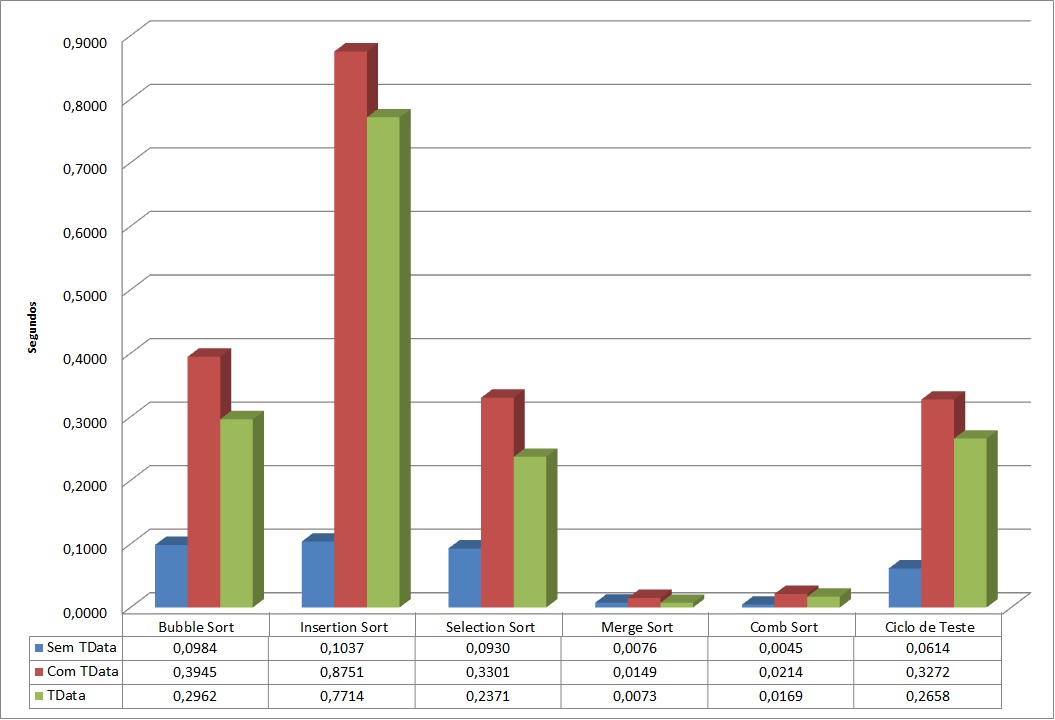
\includegraphics[width=0.9\textwidth]{figuras/tempoTData.jpg}
	\caption[Tempo de execução da Classe \textit{TData}]{O tempo de execução dos algoritmos sem a classe \textit{TData} foi relativamente baixo, sendo que o maior tempo atingiu 0,1037 segundos ou 103,7 milisegundos para ordenar um vetor de 1024 elementos. Já o tempo dos algoritmos com a Classe \textit{TData} foi um pouco maior, sendo o tempo de execução do algoritmo insertion sort que atingiu 0,8751 segundos ou 875,1 milisegundos. O tempo de execução médio da classe \textit{TData} para cada algoritmo de ordenação foi de 0,2658 segundos ou 265,8 milisegundos.}

	\label{Img:tempoTData}	
	%width=0.5\textwidth (Tamanho da Imagem)
\end{figure}

\begin{figure}[h]
	\centering
	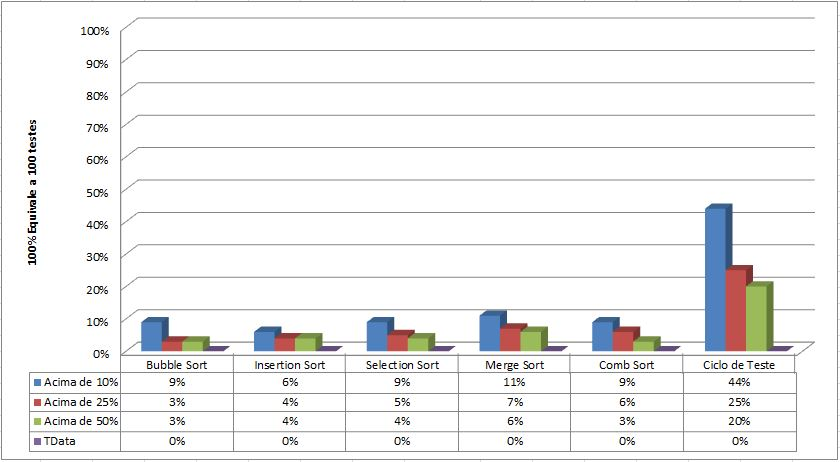
\includegraphics[width=0.9\textwidth]{figuras/falhaTData.jpg}
	\caption[Teste de redundância de dados da classe \textit{TData}]{Nesta figura para as falhas detectadas acima de 10\%, 25\% e 50\% são do teste que não utiliza redundância de dados, por exemplo, para as falhas acima de 10\%, aproximadamento 44\% dos ciclos de testes falharam. No entanto para o teste que utilizou a redundância de dados, nenhum algoritmo de ordenação ou ciclo de teste falharam. Embora o teste estivesse sendo bombardeado por falhas, a classe TData se mostrou eficaz corrigindo os valores alterados nos endereços de memória cobertos pela redundância de dados.}
	\label{Img:falhaTData}	
	%width=0.5\textwidth (Tamanho da Imagem)
\end{figure}

\newpage
\section{Recuperação de falhas da biblioteca \textit{FaultRecovery}}\label{Sec:recupeFault}

Nesta seção são mostrados os resultados dos testes realizados com a biblioteca \textit{FaultRecovery}. O código utilizado na seção \ref{Sec:tempoRecovery} foi modificado para injetar falhas em endereços de memória aleatórios. Foram utilizados os mesmos algoritmos de ordenação, no entanto o tempo de execução da biblioteca foi desprezado, pois o resultado avaliado neste teste foi a capacidade de recuperação de falhas. Se as falhas registradas nos resultados ocorressem em uma situação real, os dados afetados por essas falhas poderiam ocasionar o travamento do \textit{firmware}. Caso utilizado o mecanismo de \textit{watchdog} para a detecção de falhas, quando o \textit{whatchdog} percebesse que o microcontrolador estivesse travado, o \textit{mbed} seria reinicializado. No entanto, considerando-se o exemplo de uma estação meteorológica, se o travamento ocorresse no momento em que os dados coletados fossem enviados para um servidor remoto, por ser uma máquina de estados, no qual a ordem de execução de cada estado implica nos resultados obtidos, quando o \textit{mbed} fosse reinicializado, o primeiro estado que seria executado, poderia ou não ser o estado responsável que enviaria os dados ao servidor remoto.

Para que isso não venha a ocorrer, a estação meteorológica poderia ser implementada utilizando a biblioteca \textit{FaultRecovery} para que pontos de recuperação de falhas pudessem ser criados, para assim que o microcontrolador reinicializasse por conta de alguma falha, algum ponto de recuperação predefinido pudesse ser executado. Entretanto utilizou-se algoritmos de ordenação para simular uma máquina de estados. Foram criados pontos de recuperação para cada algoritmo de ordenação, se em algum momento o microcontrolador vier a travar e posteriormente ser reiniciado, seja manualmente ou automaticamente, o ponto de recuperação predefinido será executado. Mostra-se na figura \ref{Img:testeFaultRecovery} os resultados obtidos após a execução de cem ciclos de testes, cada ciclo é representado pela execução dos cinco algoritmos de ordenação conforme descrito na seção \ref{Sec:tempoRecovery}. 


\begin{figure}[h]
	\centering
	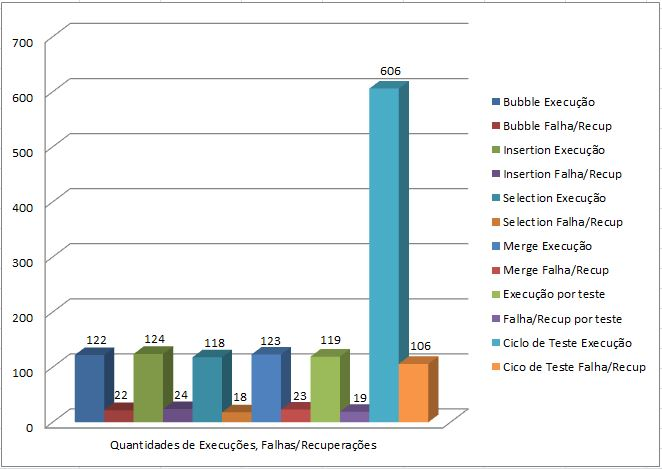
\includegraphics[width=0.9\textwidth]{figuras/testeFaultRecovery.jpg}
	\caption[Resultados Obtidos da Biblioteca \textit{FaultRecovery}]{Esta figura mostra a quantidade de execuções e falhas de cada algoritmo, inclusive de cada ciclo de teste. Por exemplo, a primeira coluna, da esquerda para e direita, representa o número de execuções do algoritmo \textit{bubble sort}, pode-se perceber que embora tenham sido executados cem ciclos de teste, o algoritmo foi executado cento e vinte e duas vezes. Em contra partida, na segunda coluna, que representa a quantidade de vezes em que um ponto de recuperação do \textit{bubble sort} foi executado, o \textit{firmware} reinicializou e executou o ponto de recuperação do \textit{bubble sort} vinte e duas vezes.}
	\label{Img:testeFaultRecovery}	
	%width=0.5\textwidth (Tamanho da Imagem)
\end{figure}


\section{Injeção de Falhas com a Biblioteca \textit{FaultInjector}}

Esta seção mostra o resultado de injeção de falhas na memória \textit{flash} do microcontrolador \textit{mbed} LPC1768. A injeção de falhas na memória \textit{flash} sorteou um setor aleatório para injetar uma quantidade predefinida de falhas, que podem variar de 256, 512, 1024 ou 4096 bytes. Na figura \ref{Img:injecaoFlash} é exibido um teste em que foram injetadas 256 bytes de falhas no setor 25, que foi sorteado aleatoriamente pelo injetor de falhas. O endereço de memória do setor sorteado em hexadecimal inicia em 0x00058000 e termina em 0x0005FFFF. Pode-se perceber que os bytes dos endereços de memória do setor 25 (0x00058000 até 0x000580F0) foram alterados.

\begin{figure}
	\centering
	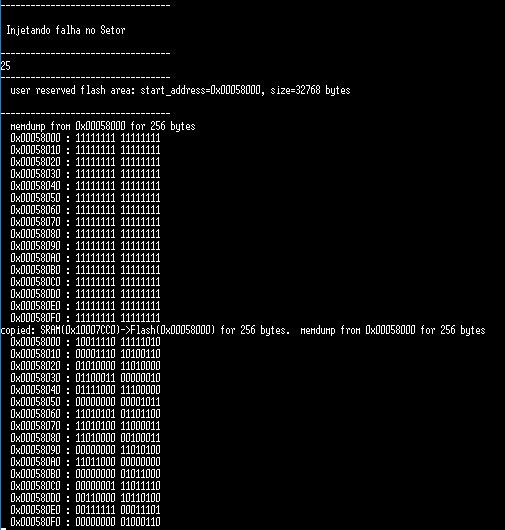
\includegraphics[width=0.9\textwidth]{figuras/injecaoFlash.jpg}
	\caption[Injeção de Falhas na Memória \textit{Flash}]{Nesta figura é mostrado o setor da memória \textit{flash} soteado pelo injetor de falhas e os endereços desse setor. Além de mostrar como os bits se encontravam antes de serem modificados, assim como também pode ser visualizada a modificação desses bits.}
	\label{Img:injecaoFlash}	
	%width=0.5\textwidth (Tamanho da Imagem)
\end{figure}